\section{Xamarin}
\label{sec:Frameworks_Xamarin}

Das von Microsoft entwickelte Xamarin-Framework setzt auf die .NET Technologie und ermöglicht die plattformübergreifende App-Entwicklung in C\# und die Nutzung der im Framework .NET enthaltenen Funktionen.
Neben Android und iOS kann der gleiche Code auch für Windows-Anwendungen verwendet werden.
Laut Microsoft können „bis zu 90 \% des Codes“ \cite{Xamarin_Homepage} wiederverwendet werden.
Dazu werden häufig verwendete Funktionen über eine gemeinsame abstrakte Schnittstelle bereitgestellt und ein Großteil der Funktionen der Plattform-\acp{SDK} können über Bindings in C\# aufgerufen werden.
Dennoch ist es für komplexe Anwendungsfälle möglich, Bindings für native Bibliotheken zu erstellen.
So lassen sich neben vorhandenen Bibliotheken auch neue benutzerdefinierte Bibliotheken erstellen, womit beliebiger nativer Code in eine Xamarin-App eingebunden werden kann \cite{Xamarin_Android}.


Zur Ausführung von .NET-Code auf den mobilen Plattformen, wird die Mono Ausführungsumgebung verwendet, eine Open-Source Runtime für .NET.
Parallel kommt jeweils eine native Ausführungsumgebung zum Einsatz, welche die Verwendung von Plattform-\acp{API} und die Interoperabilität mit nativem Code ermöglicht.
Unter Android wird hierfür die \ac{ART} verwendet, unter iOS die Objective-C Ausführungsumgebung \cite{Xamarin_iOS,Xamarin_Android}.
Die sich ergebende Architektur ist in \autoref{fig:xamarin_architecture} dargestellt.
\begin{figure}[h]
    \centering
    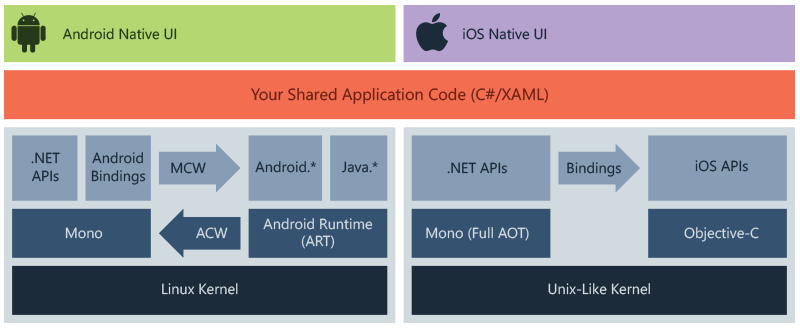
\includegraphics[width=\textwidth]{xamarin_architecture.png}
    \caption{Architektur einer Xamarin-App \cite{Xamarin_Homepage}.}
    \label{fig:xamarin_architecture}
\end{figure}


Durch die Verwendung von C\# ist Xamarin nach Nunkessers Taxonomie \cite{Nunkesser_Taxonomy_Apps} eine Foreign Language App.
Um die Verwendung von C\# unter Android und iOS zu ermöglichen, wird der Code zunächst mithilfe des Open-Soruce Mono-Compilers in das Zwischencodeformat \ac{MSIL} kompiliert.
Normalerweise wird dieser Code beim Anwendungsstart von der .NET \ac{CLR} mit einem \ac{JIT}-Compiler zu Plattformspezifischem Code kompiliert.
Für iOS-Anwendungen wird der \ac{MSIL}-Code jedoch \ac{AOT} kompiliert, da Apple unter iOS die Ausführung von dynamisch erzeugtem Code aus Sicherheitsgründen nicht erlaubt \cite{Xamarin_iOS}.
Der Buildprozess einer Xamarin-Anwendung mit den beiden Zielplattformen Android und iOS ist in \autoref{fig:xamarin_build} dargestellt.
Durch die \ac{AOT}-Kompilierung Unterscheiden sich Xamarin-Apps unter iOS von Xamarin-Apps unter Android.
Zum Beispiel ist die Startzeit einer Anwendung unter iOS durch den Wegfall der \ac{JIT}-Kompilierung beim Start signifikant kürzer.
Allerdings gibt es auch Einschränkungen, wie beispielsweise das Fehlen einiger Reflection-Funktionen, welche bei der Entwicklung beachtet werden müssen \cite{Xamarin_iOS,Xamarin_iOS_Limitations}.
\begin{figure}[h]
    \centering
    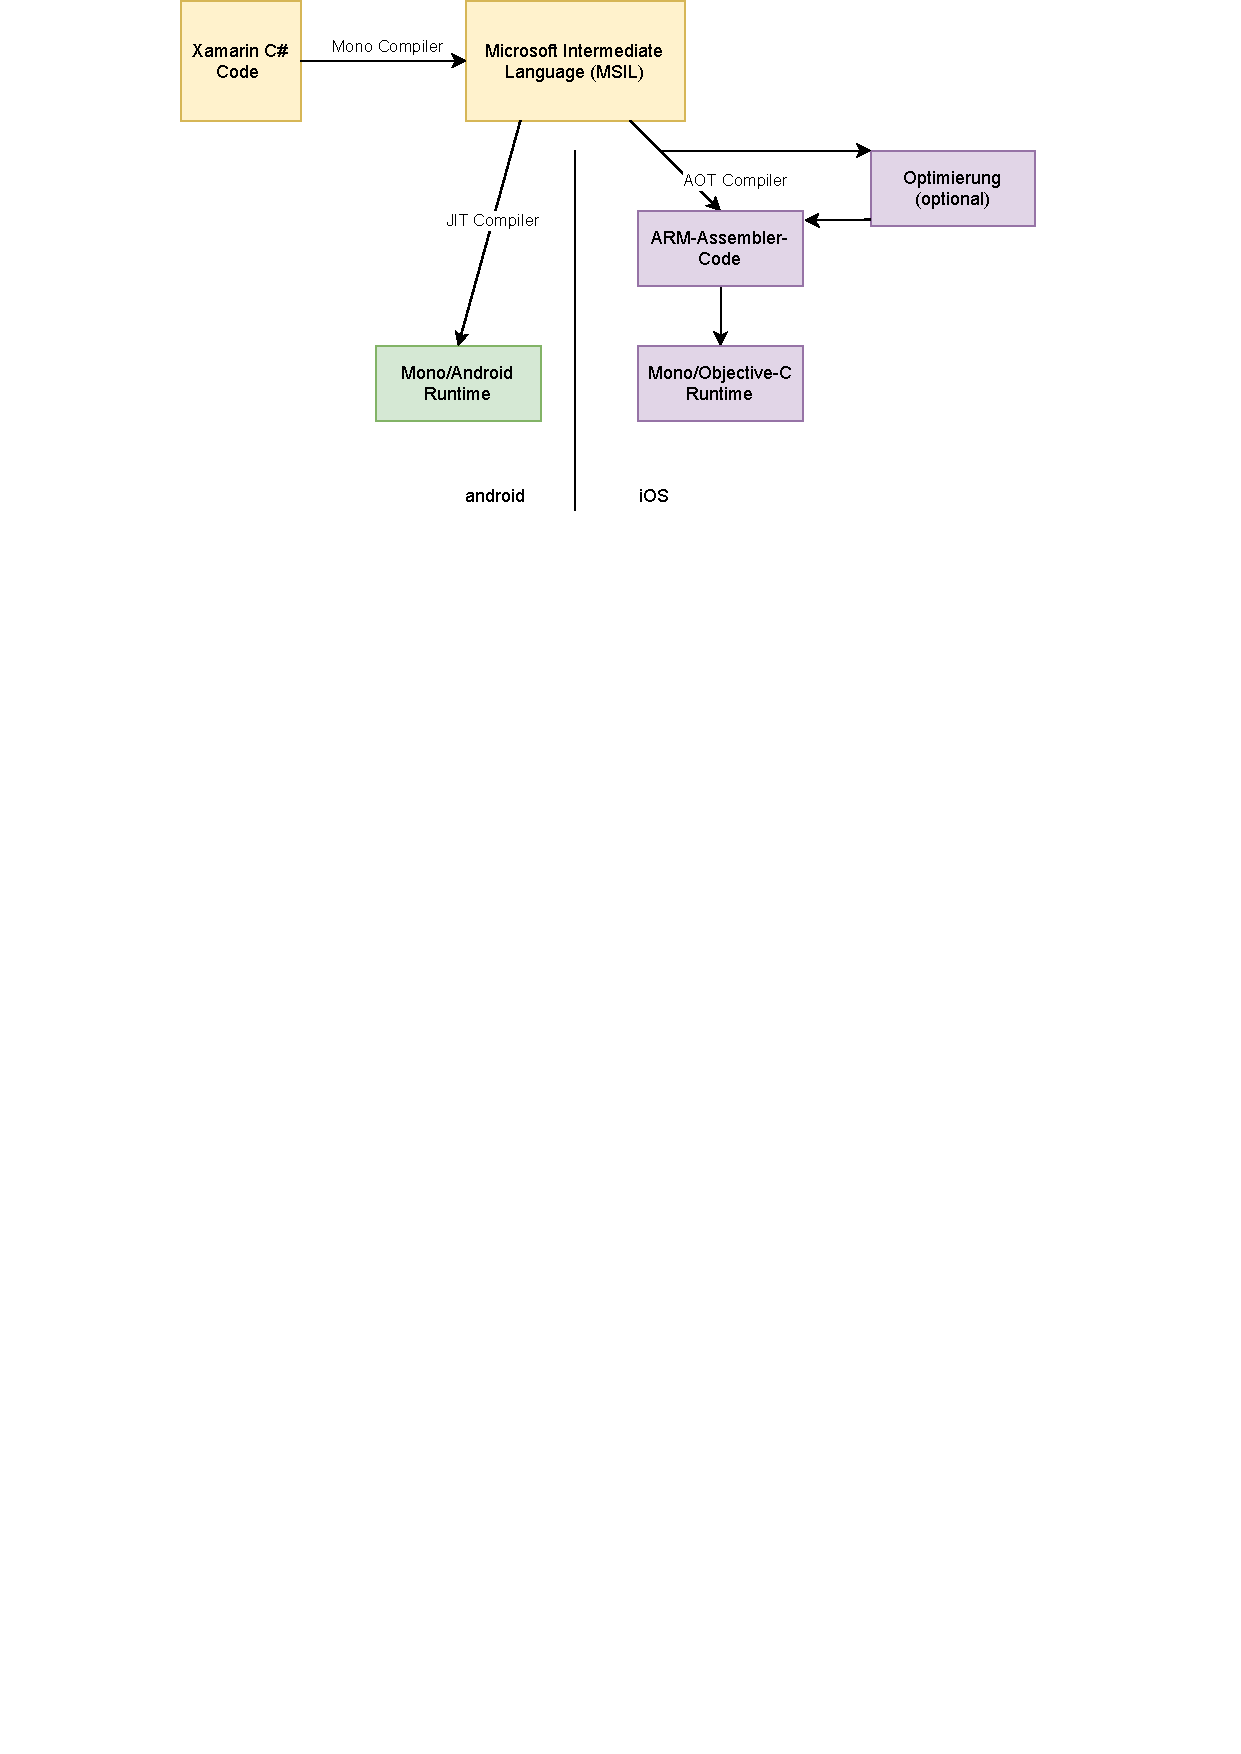
\includegraphics[clip, trim=3cm 20cm 0 0, width=1.2\textwidth]{xamarin_build.pdf}
    \caption{Buildprozess einer Xamarin-Anwendung für die Plattformen Android und iOS.}
    \label{fig:xamarin_build}
\end{figure}


Ein großes Problem von Xamarin besteht darin, dass typischerweise für jede Plattform eine eigene native Benutzerschnittstelle entwickelt werden muss, wie auch in \autoref{fig:xamarin_architecture} gezeigt \cite{Xamarin_Homepage}.
Das erhöht den Aufwand im Vergleich zu anderen Frameworks, welche standardmäßig eine plattformübergreifende Benutzerschnittstelle bereitstellen.
Deshalb bietet Xamarin mit der \ac{UI}-Bibliothek Xamarin.Forms eine Erweiterung zur plattformübergreifenden Entwicklung von Oberflächen \cite{Xamarin_Homepage}.
Auf der Konferenz Microsoft Build, hat das Unternehmen 2020 angekündigt das Xamarin-Framework besser in .NET zu integrieren und im Zusammenhang die Bezeichnung Xamarin abzuschaffen.
Stattdessen werden die Komponenten Xamarin.Android und Xamarin.iOS zu .NET for Android und .NET for iOS umbenannt, wobei die darunterliegende Technologie erhalten bleibt \cite{MS_Build_2020}.
Xamarin fließt damit komplett in .NET ein und ist nicht mehr als eigenständiges Framework zu betrachten.
Der Support für Xamarin endet am ersten Mai 2024 \cite{Xamarin_EOL}.
Als Nachfolger für Xamarin wurde auf der Microsoft Build 2020 das Framework .NET \ac{MAUI} angekündigt.
Der Namen verdeutlicht einen starken Fokus auf plattformübergreifende Entwicklung von Benutzerschnittstellen, weshalb .NET \ac{MAUI} auch als Weiterentwicklung von Xamarin.Forms angesehen wird \cite{NET_MAUI_Introduction}.
Allerdings übernimmt das Framework auch die Abstraktion der verschiedenen .NET Implementierungen auf den einzelnen Zielplattformen und wir von Microsoft explizit als Cross-Plattform Framework beworben \cite{NET_MAUI}.
Technisch kann .NET \ac{MAUI} daher als Weiterentwicklung von Xamarin betrachtet werden und beide Bezeichnungen lassen sich in vielen Fällen synonym verwenden.
Da die erste Version von .NET \ac{MAUI} erst im Mai 2022 veröffentlicht wurde \cite{NET_MAUI_Release}, wird in dieser Arbeit weiterhin von Xamarin gesprochen.
% TODO: wird später MAUI verwendet oder nicht, eventuelle Unterschiede


Xamarin-Anwendungen weisen allgemein eine hohe Performance auf, in einigen Fällen wird eine Performance wie bei nativen Anwendungen erreicht \cite{Nawrocki_Comparison_Hybrid_Native_Frameworks, Bakker_Xamarin_XamarinForms_Native, Xamarin_Homepage}.
Durch die \ac{JIT}-Kompilierung und Android kann die Startzeit jedoch vergleichsweise lang ausfallen \cite{Willocx_CrossPlatform_Performance}.
Unter iOS ist dieser Nachteil nicht gegeben, allerdings sind dafür die Apps um einiges größer als nativ entwickelte Apps.
Nawrocki \textit{et al.} \cite{Nawrocki_Comparison_Hybrid_Native_Frameworks} berichten von einem bis zu 16-fachen Speicherbedarf.

In der Stackoverflow-Umfrage 2022 \cite{Stackoverflow_2022} gibt eine Mehrheit von 61,47 \% der Entwickler, die bereits mit Xamarin gearbeitet haben, an, das Framework nicht weiterhin verwenden zu wollen.
Bis auf Cordova schneiden alle anderen, in dieser Arbeit untersuchten Cross-Plattform Frameworks besser ab.
Inwiefern die Beliebtheit auf Probleme bei der Benutzung oder beim Zugriff auf Gerätefunktionen zurückzuführen ist, wird sich im Laufe dieser Arbeit zeigen.